This appendix includes derivation of the bernoulli equation (\autoref{eq:bernoulli}) and the expression for the input work to the solution pump (\autoref{eq:pump:Wsop}).
\subsection{Bernoulli Equation}
Consider at pipe with two pressure differences at depicted at \autoref{fig:app:bernold}.
\begin{figure}[H]
	\centering
		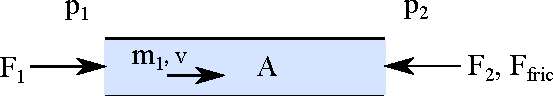
\includegraphics[width=0.45\textwidth]{appendices/pictures/bernoulli.pdf} 
		\caption{A pipe with two different pressures and a mass flow inside.}
	\label{fig:app:bernold}
\end{figure}
Applying Newtons second law:
\pp
F_\text{res} = F_1 - F_2 - F_\text{fric}
\label{eq:app:pump:res}
\end{flalign}
As:
\pp
&F_\text{res} = M\,a = 0 \kk \text{The solution pump is only considered in steady state $\Rightarrow a=0$ } \nonumber \\
&F_1 = p_1\,A \nonumber \\
&F_2 = p_2\,A \nonumber \\
&F_\text{fric} = c_x\,v^2 \nonumber
\end{flalign}
Hence \autoref{eq:app:pump:res} can be written as:
\pp
0 =  p_1\,A - p_2\,A - c_x\,v\,|v|
\end{flalign}
By considering units, $v$ may be expressed as:
\pp
v = \dfrac{m_1}{\rho_1\,A} \label{app:pump:v}
\end{flalign}
Inserting \autoref{app:pump:v} in \autoref{eq:app:pump:res} and some rearrangement:
\pp
&0 = p_1\,A - p_2\,A - c_x\, \dfrac{m_1}{\rho_1\,A} \, \left| \dfrac{m_1}{\rho_1\,A} \right| \kk \Leftrightarrow \\
&0 = A(p_2 - p_1) - c_x\, \dfrac{m_1}{\rho_1\,A} \, \left| \dfrac{m_1}{\rho_1\,A} \right| \kk {\scriptstyle \text{density and area are always positive} \above0pt \Leftrightarrow } \\
&0 = \rho_1^2\, A^3(p_2 - p_1) - c_x\,m_1|m_1| \kk \Leftrightarrow \nonumber \\
&\rho_1^2\, A^3(p_2 - p_1)  = c_x\,m_1|m_1| \kk \Leftrightarrow \nonumber \\
& \rho_1 (p_2 - p_1) = c_y\,m_1|m_1| \kk  { \scriptstyle \text{$c_y = c_\text{SO,P}$}  \above0pt \rightarrow } \kk \rho_1 (p_2 - p_1) = c_\text{SO,P}\,m_1|m_1| \label{eq:app:bern:final}
\end{flalign}
\subsection{Flange Power (input work)}
First, consider the scenario depicted in \autoref{fig:app:lolol}. A pressure, $p$, causes the circle to be displaced by a small distance $dx$
\begin{figure}[H]
	\centering
		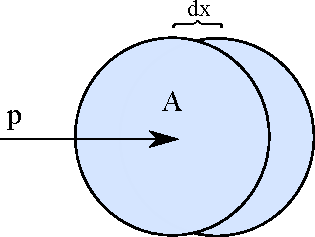
\includegraphics[width=0.25\textwidth]{appendices/pictures/work_app.pdf} 
		\caption{.}
	\label{fig:app:lolol}
\end{figure}
This give rise to a force, $F$:
\pp
F = p\cdot A \nonumber
\end{flalign}
This force may also be expressed by some work in a small amount of time:
\pp
W\,\Delta \, t = F\,\Delta x \kk \Leftrightarrow \kk W\,\Delta \, t = p\,\underbrace{ A\,\Delta x }_{\Delta V} \kk \Leftrightarrow \kk W\, \Delta \, t = p \Delta \, V \nonumber
\end{flalign} 
Where $V$ is the volume. By dividing by $\Delta \, t$:
\pp
W = p\,\dfrac{\Delta  V}{\Delta \, t}\nonumber
\end{flalign}
Where $\Delta V/ \Delta \, t$ is the change in volume (volumetric flow). The volumetric flow can also be expressed as $m/\rho$ such that:
\pp
W = p\,\dfrac{m}{\rho} \nonumber
\end{flalign}
Now, as the control volume is between two different pressures (which it indeed is) it can be expressed as:
\pp
W = (p_2 - p_1)\, \dfrac{m}{\rho} \nonumber
\end{flalign}
Adding the pump efficiency to the equation:
\pp
\eta\,W = (p_2 - p_1)\dfrac{m}{\rho}
\end{flalign}
Which is the model used in the solution pump modelling (\autoref{sec:pump}, \autoref{eq:pump:Wsop})